\chapter{Speichersysteme in Videospielen}\label{ch:videospiele}
\iffalse
Email an Entwicklern:\\
\\
Dear <Game Studio>,\\
I am a student at the University of Kassel in Germany and I am currently working on my bachelor's thesis about saving and loading systems for video games. For my thesis I want to find out, how the user's game data (player position, items, blocks from the game world, enemies, ...) can be efficiently saved and eventually loaded. In one chapter of my thesis, I want to look at popular games and how they have implemented their saving and loading systems. As the game <Game Name> has a lot of data, that needs to be saved efficiently, it would be very helpful for my thesis, if you could look at my following questions about your game.

\begin{enumerate}
    \item Which different Datatypes does your game have (e.g. Player Data, Item Data, Block Data, ...). What does each Datatype store?
    \item Which folders and files does the save folder have and what data are saved in each folder?
    \item Which format do the game files have to save each data? (e.g. JSON-Format)
    \item Is the data split up in some way or is everything saved all together in one big collection? If the data is split up into multiple sections, how is it split (e.g. chunk-system to divide the data)?
    \item Is the data saved compressed? 
    \item Which phases does the saving of the game have? What data is saved when? Does the game use auto-save and if yes when?
    \item Which phases does the loading of the game have? Is every data loaded at once or only the needed data? When is the rest of the data loaded?
\end{enumerate}

Thanks for your attention. I’m looking forward to your reply,\\
Giulio Pazzi
\fi
%--------------------------------------------------------------------------


%--------------------------------------------------------------------------
\section{Minecraft}
Zusammenfassung über Minecraft (Für Leute die das Spiel nicht kennen).
\begin{itemize}
    \item Survival Spiel
    \item 3D Welt die aus Blöcken besteht
    \item Unter meistgespielten Spielen
\end{itemize}

In diesem Kapitel wurde die Minecraft Version 1.16 angeschaut. 
Bei neueren Versionen kann das Speichersystem bereits etwas anders aussehen. Um an den Sourcecode zu kommen wurde das Tool 
\url{https://github.com/Hexeption/MCP-Reborn/tree/1.16} verwendet. Aus rechtlichen Gründen darf kein
Sourcecode gezeigt werden.

\subsection{Daten}
Welche Klassen gibt es bei Minecraft (Blöcke, Chunks,...) und welche Daten 
beinhalten diese.\\
\\
Blöcke mit YZX Position (einfacher zu komprimieren), "BlockStates", etc.\\
BlockState über "Palette" Liste gespeichert (Welche BlockIDs welchen Zustand haben).\\
$\Rightarrow{}$ ChunkSerializer.java:write()\\

Entity (z.B. Player) mit ID, Position, Motion, Rotation, OnGround, CustomName, ...\\
$\Rightarrow{}$ Entity.java:writeWithoutTypeID()\\

\url{https://minecraft.fandom.com/wiki/Chunk_format}

\subsection{Ordnerstruktur}
Ordner:
\begin{itemize}
    \item /world/data
    \item /world/players: Player Data
    \item /world/DIM-1: Nether world
    \item /world/DIM1: End world
    \item /world/region: Overworld regions
    \item /world/DIM-1/region: Nether regions
    \item /world/DIM1/region: End regions
\end{itemize}

Dateien:
\begin{itemize}
    \item level.dat: Allgemeine Spieldaten
    \item $[$playeruuid$]$.dat: Spielerdaten
    \item $[$region$]$.mca: Regionen in /region Ordner
\end{itemize}

\url{https://wiki.vg/Map_Format}\\
\url{https://minecraft.fandom.com/wiki/Java_Edition_level_format}

\subsection{Speicherformate}
\begin{itemize}
    \item Minecraft Anvil (MCA): Speichern von Chunk Daten (RegionFileCache.java:loadFile(), SaveFormat.java:convertRegions())
    \item Named Binary Tag (NBT): .dat-Endung $\Rightarrow$ level.dat, Playerdata, ... (CompoundNBT in vielen Dateien und NBT Folder)
    \item JavaScript Object Notation (JSON): Speichern von Texte (Bücher, Schilder, Label)
\end{itemize}

\url{https://docs.fileformat.com/game/mca/}\\
\url{https://wiki.vg/NBT}\\
\url{https://minecraft.fandom.com/wiki/JSON}

\subsection{Datenaufteilung}
Chunks, Regions und Level. 

\begin{itemize}
    \item Section: Bereich von 16x16x16-Blöcken
    \item Chunk: Bereich von 16x16x$[$Welt Höhenlimit$]$ Blöcken (Bei Minecraft 1.16 Höhenlimit = 256 $\Rightarrow{}$ Chunk = 16xSections (Chunk.java:sections))
    \item Region: Gruppierung von Chunks in einem 32x32 Blöcke Gebiet
    \item Level: (Theoretisch, aber nicht praktisch) unendliche Sammlung von Chunks gespeichert als regions
\end{itemize}

\url{https://minecraft.fandom.com/wiki/Chunk_format}
\url{https://wiki.vg/Region_Files}

\subsection{Speichervorgänge}

Speicherung, wenn:
\begin{itemize}
    \item Neue Welt generiert (Minecraft.java:createWorld())
    \item Pause-Taste wird gedrückt (IntegratedServer.java:tick())
    \item Chunks werden entladen (Spieler zu weit weg)
    \item Alle 5 Minuten
\end{itemize}

\url{https://minecraft.fandom.com/de/wiki/Spielstand-Speicherung}

\subsection{Ladevorgänge}
%--------------------------------------------------------------------------



%--------------------------------------------------------------------------
\section{Factorio}
\begin{enumerate}
    \item Ressourcen minen 
    \item Technologien forschen
    \item Infrastruktur aufbauen
    \item Automatisieren von Produktion
    \item Gegner bekämpfen
    \item In Lua geschrieben
\end{enumerate}
\url{https://www.factorio.com/}

Allgemein benutzt Factorio ein "Deterministic save load"
\url{https://gist.github.com/Rseding91/a309cf0a30782a2e96ef081c39326f42}

\wichtig{Quelle mit Email nennen}

\subsection{Daten}

\begin{figure}[htp]
    \centering
    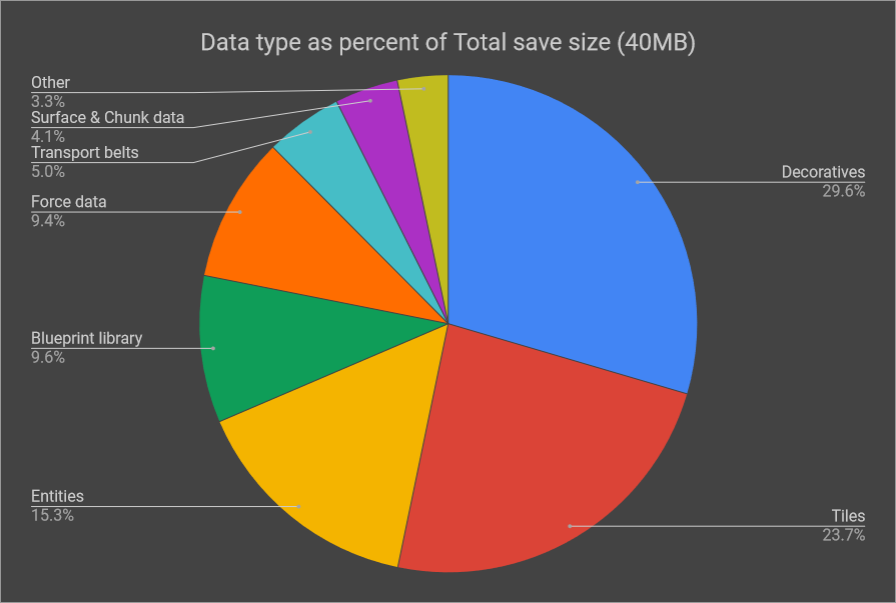
\includegraphics[width=0.8\textwidth]{images/factorio_save_statistic.png}
    \caption{Anteil der Datentypen beim Speichern}
    \label{fig:factorioSaveStatistic}
\end{figure}
% 27.7.2023
\url{https://www.factorio.com/blog/post/fff-270}

Map Daten bestehen aus:
\begin{itemize}
    \item Dekorative Spielobjekte 
    \item Tiles 
    \item Entitäten
    \item Blueprint Library
    \item Physikalische Kräfte
    \item Transportband
    \item Oberfläche und Chunk Daten
    \item Weitere Daten...
\end{itemize}

\subsection{Ordnerstruktur}

\subsection{Speicherformate}

\subsection{Datenaufteilung}

\subsection{Speichervorgänge}
Kurzgefasst:
\begin{enumerate}
    \item ID Mapping speichern (\url{https://www.factorio.com/blog/post/fff-259})
    \item Map Daten speichern
\end{enumerate}

Detaillierter:
\begin{enumerate}
    \item Volles leeren der Garbage Collection von allen Lua Zuständen
    \item Löschen von temporären Map Daten, die während des Speicherprozesses entstanden sind
    \item ID mapping speichern (ID mapping für alles was IDs benutzt)
    \item Speichern der Prototypenmigrationen
    \item Rest, der gespeichert weden soll, abspeichern
    \item SaveHelpers speichern
\end{enumerate}
\url{https://gist.github.com/Rseding91/a309cf0a30782a2e96ef081c39326f42}

\subsection{Ladevorgänge}
Kurzgefasst:
\begin{enumerate}
    \item Map Version überprüfen
    \item Überprüfen ob Mods hinzugefügt/gelöscht/verändert wurden
    \item invalide/korrupte save files finden 
\end{enumerate}

Detaillierter:
\begin{enumerate}
    \item Map-Version überprüfen (save file map und die map in der die save file map geladen wird)
    \item Überprüfen, ob aktive Mods oder die Mod-Einstellungen sich verändert haben (wenn ja, müssen Aktionen nach dem laden durchgeführt werden) und setze flag wenn das der Fall ist
    \item ID mapping laden
    \item Angewandte Migrationen laden und nicht angewandte Migrationen ausführen
    \item Standard Map Daten laden (Enitäten, Chunks, Forces, Züge)
    \item load in allen LoadHelpers aufrufen
    \item Inszenierte (???) Veränderungen ausführen
    \item Enitäten, die Ladeprobleme hatten, nachladen
    \item Targeters wiederherstellen
    \item setup bei allen LoadHelpers ausrufen
    \item Wenn Prototyp Daten verändert wurden Elektrisches Netz Daten clearen
    \item setup aller transport belt connectible Entitäten aufrufen
    \item Ruf setup von Entität auf, wenn diese während Laden erstellt wurde und nicht existierte, als die Map zuletzt gespeichert wurde
    \item postLoadHook für die Map aufrufen
    \item Tile Probleme fixen, nachdem alle Enitäten geladen wurden und setup fertig ist
    \item Ruf bei allen PreFinalLoadHelper setup auf
    \item Ruf bei allen FinalLoadHelper setup auf
    \item Für alle Oberflächen postSetup aufrufen
    \item Lua Daten laden und wiederherstellen
    \item "configuration changed" Lua event ausführen
\end{enumerate}
%--------------------------------------------------------------------------


%--------------------------------------------------------------------------
\section{Terraria}
\subsection{Daten}
Welche Klassen gibt es bei Terraria (Blöcke, Chunks,...) und welche Daten 
beinhalten diese.

\subsection{Ordnerstruktur}

\subsection{Speicherformate}
World-Dateien, Player-Dateien, Konfigurationsdateien 

\subsection{Datenaufteilung}
Kein Chunksystem, alles in einer Datei gespeichert. Aber Inventar, Position
usw. werden in verschiedenen Daten gespeichert.

\subsection{Speichervorgänge}

\subsection{Ladevorgänge}
%--------------------------------------------------------------------------


%--------------------------------------------------------------------------
\iffalse
\section{Ein Spiel}
Beschreibung von dem Spiel

\subsection{Daten}
Welche Klassen gibt es bei <Spielname> (Blöcke, Chunks,...) und welche Daten 
beinhalten diese.

\subsection{Ordnerstruktur}

\subsection{Speicherformate}

\subsection{Datenaufteilung}

\subsection{Speichervorgänge}

\subsection{Ladevorgänge}
\fi
